\documentclass[a4paper,12pt]{article}
\usepackage[dutch]{babel}
\usepackage{geometry}
\geometry{a4paper, margin=1in}
\usepackage{graphicx}
\usepackage{hyperref}
\usepackage{array}
\usepackage[table,xcdraw]{xcolor}
\usepackage{lipsum}
\usepackage{tikz}
\usetikzlibrary{arrows.meta, positioning}

\geometry{a4paper, top=4cm, bottom=3.5cm, left=2.5cm, right=2.5cm} 


\setlength{\parskip}{0.8em}
\setlength{\parindent}{0pt}

\usepackage{hyperref}
\hypersetup{
    colorlinks=true,      % false: boxed links; true: colored links
    linkcolor=black,       % color of internal links
    citecolor=black,       % color of links to bibliography
    filecolor=black,    % color of file links
    urlcolor=blue      % color of external links
}
\urlstyle{same}           % Use normal text font for URLs

\raggedright
\sloppy

\title{}
\author{}
\date{}

\begin{document}

\begin{titlepage}
    \centering
    \vspace*{0cm}
    \LARGE{Profielwerkstuk Voorstel:} \\
    \Huge\textbf{Reinforcement Learning en Computerspellen} \\
    \vspace{1.5cm}
    \rule{\linewidth}{0.4mm}
    \Large
    Hoe beïnvloeden de specifieke kenmerken van computerspellen de effectiviteit van verschillende reinforcement learning-algoritmes in het optimaliseren van spelprestaties? \\
    \rule{\linewidth}{0.4mm} \\
    \vspace{1.5cm}
    
\includegraphics[width=0.2\textwidth]{logo-clz.png} \\
    \vspace{\fill}
    \large
    \textbf{Matthijs Gorter} \\
    \textbf{Thom Brinkhorst} \\
    \textbf{Pepijn van Iperen} \\
    \vspace{\fill}
    \normalsize

    Profielwerkstuk \\ onder begeleiding van \\ \textit{\textbf{S. Rook}} \\
    Christelijk Lyceum Zeist \\ Natuur en Techniek \\ 6 september 2024 \\ \newpage
\end{titlepage}
\section{Doel van het onderzoek}
Het doel van dit onderzoek is om te begrijpen hoe de kenmerken van
verschillende computerspellen de effectiviteit van verschillende reinforcement
learning (RL) algoritmes beïnvloeden bij het verbeteren van spelprestaties. Dit
onderzoek richt zich op het identificeren van de eigenschappen van
verschillende soorten spellen en de kenmerken van RL-algoritmes.

Door verschillende RL-algoritmes toe te passen op een reeks spellen met
verschillende kenmerken, willen we ontdekken welke algoritmes het beste
presteren in welke soorten spellen. Dit kan variëren van strategische spellen
die planning vereisen tot actiespellen die snelle beslissingen vragen.
\section{Onderzoeksvragen}
\subsection{Hoofdvraag}
Hoe beïnvloeden de specifieke kenmerken van computerspellen de effectiviteit
van verschillende reinforcement learning-algoritmes in het optimaliseren van
spelprestaties?
\subsection{Deelvragen}
Om beter te begrijpen hoe de kenmerken van computerspellen de prestaties van
verschillende reinforcement learning (RL) algoritmes beïnvloeden, hebben we
drie belangrijke deelvragen opgesteld
\begin{enumerate}

    \item\subsubsection*{Wat zijn de specifieke kenmerken van verschillende soorten computerspellen?}
          Deze vraag richt zich de eigenschappen van
          verschillende soorten computerspellen. Spellen kunnen sterk verschillen in
          hoe ze zijn opgebouwd, hoe snel spelers beslissingen moeten nemen en hoe
          complex de spelregels zijn. Door deze kenmerken te onderzoeken, kunnen
          we inzicht krijgen in welke aspecten van een spel een uitdaging vormen voor RL-algoritmes.

    \item\subsubsection*{Welke reinforcement learning-algoritmes zijn beschikbaar en wat zijn hun
              kenmerken?}
          Hier willen we kijken naar de verschillende soorten RL-algoritmes die beschikbaar
          zijn en wat hen uniek maakt. Sommige algoritmes zijn beter in het leren van eenvoudige
          taken, terwijl andere juist goed zijn in het omgaan met complexe situaties.

    \item\subsubsection*{Hoe beïnvloeden de spelkenmerken de prestatie van
              reinforcement learning-algoritmes?}

          Deze vraag gaat in op het belangrijkste deel van het onderzoek: het verband
          tussen de kenmerken van een spel en hoe goed een RL-algoritme presteert. We
          willen weten hoe bepaalde eigenschappen van een spel, zoals de noodzaak voor
          snelle beslissingen of lange-termijnplanning, invloed hebben op de
          effectiviteit van een algoritme. Door de prestaties van verschillende
          algoritmes in verschillende spellen te vergelijken, kunnen we ontdekken welke
          het beste werken voor bepaalde soorten spellen en waarom dat zo is.

\end{enumerate}
\section{Experimenten}
In dit onderzoek willen we kijken hoe verschillende reinforcement learning (RL)
algoritmes presteren in verschillende computerspellen. We hebben drie spellen
gekozen: Snake, Schaken, en Mario Super Bros. Elk spel heeft zijn eigen
kenmerken en uitdagingen, en we zullen drie RL-algoritmes testen: Deep
Q-Network (DQN), Proximal Policy Optimization (PPO), en AlphaZero (of Deep
Deterministic Policy Gradient (DDPG) als AlphaZero niet lukt). Het doel is om
te ontdekken hoe goed elk algoritme werkt in elk spel en hoe de kenmerken van
het spel de prestaties van de algoritmes beïnvloeden.
\subsection*{Experiment 1: Snake} Snake is een simpel actiespel waar je een slang bestuurt die appels eet om
langer te worden, terwijl je ervoor zorgt dat hij zichzelf niet raakt. Het spel
vereist snelle beslissingen en het vooruitzicht zodat je je zelf niet opsluit.
Het doel van het experiment met Snake is om te onderzoeken hoe de RL-algoritmes
presteren in een omgeving met beperkte ruimte en snel veranderende situaties.
We zullen kijken hoe snel elk algoritme leert, hoe stabiel de prestaties zijn
en wat de uiteindelijke score is. \subsection*{Experiment 2: Schaken} Schaken is een complex bordspel met een grote hoeveelheid mogelijke zetten en
uitkomsten. Dit experiment is bedoeld om te bepalen hoe de RL-algoritmes omgaan
met de grote hoeveelheid mogelijkheden en de noodzaak om
lange-termijnstrategieën te ontwikkelen. We zullen meten hoe snel de algoritmes
leren, hoe goed de strategieën zijn die ze ontwikkelen (gecontroleerd door een
schaakprogramma), en hoe consistent de prestaties zijn in verschillende
schaaksituaties.

\subsection*{Experiment 3: Mario Super Bros}
Mario Super Bros, is een platformspel waarin de speler een personage bestuurt
dat door verschillende levels moet navigeren, obstakels moet vermijden en
vijanden moet verslaan. Dit spel combineert elementen van actie en planning,
met veel variatie in speelomgevingen en uitdagingen. Het doel van het
experiment met Mario Super Bros is om te onderzoeken hoe de RL-algoritmes
presteren in een dynamische omgeving waar zowel snelheid als strategie nodig
zijn. We zullen beoordelen hoe snel de algoritmes leren, hoe stabiel de
prestaties zijn, en hoeveel levels succesvol worden voltooid.

\section{Relevantie van het Onderzoek}
Dit onderzoek laat effectiviteit van reinforcement learning algoritmes in
verschillende omgevingen laat zien, wat bijdraagt aan het beter gebruik van
AI-systemen. Deze kennis kan niet alleen worden toegepast binnen de
game-industrie, maar ook in andere sectoren zoals de gezondheidszorg,
zelfrijdende auto's en robotica.

\section{Achtergrondinformatie}
Reinforcement Learning (RL) is een tak binnen kunstmatige intelligentie waarin
een agent leert door interactie met zijn omgeving. Een agent is een entiteit
die leert en acties onderneemt. Bij een zelfrijdende auto is het
besturingssysteem de agent, en bij een schaakspel is de schaker de agent. De
omgeving is alles waarmee de agent interageert en die reageert op de acties van
de agent. Bij een zelfrijdende auto is dit de weg waar de auto op rijdt en de
voertuigen om de auto heen. Bij een schaakspel is dit het schaakbord.

De agent leert door interactie met zijn omgeving. De agent ontvangt beloningen
of straffen (negatieve beloningen) als gevolg van zijn acties. Het doel van de
agent is om een strategie te ontwikkelen die de cumulatieve beloning
maximaliseert over tijd. Bij Super Mario Bros (1985) is Mario de agent en de
agent krijgt een beloning als Mario richting de eindslag beweegt (meestal naar
rechts) en als Mario een coin of een power up oppakt en Mario krijgt een straf
als Mario sterft en hij krijgt elke seconde straf zodat hij zo snel mogelijk
het level wilt voltooien.
\subsection{Kerncomponenten van Reinforcement Learning}
Een actie naar de beslissing die een agent neemt bij elke stap in een
besluitvormingsproces. Acties worden aangeduid met \( a \) en worden gekozen
uit een reeks mogelijke acties \( \mathcal{A} \). Elke door de agent genomen
actie beïnvloedt de interactie met de omgeving, wat leidt tot een verandering
in de toestand en een daaruit voortvloeiende beloning.

Een toestand \( x \) vertegenwoordigt de huidige situatie of staat van de
omgeving waarin de agent opereert. Dit wordt aangeduid met \( x \) en maakt
deel uit van de toestandsruimte \( \mathcal{X} \). Bij de aanvangsstap \( t = 0
\), begint de agent in een initiële toestand \( x_0 \) die willekeurig wordt
bepaald door een verdeling \( p \). Naarmate het proces vordert, bevindt de
agent zich in nieuwe toestanden gebaseerd op zijn acties.

Een beloning \( r \) is een feedbackwaarde die wordt ontvangen nadat de agent
een actie heeft uitgevoerd in een bepaalde toestand. Deze beloning wordt
bepaald door de beloningsfunctie \( r(x, a) \). De beloningsmatrix \( R \)
bevat de onmiddellijke beloningen voor elke combinatie van toestand en actie.

Een overgang beschrijft de verandering van de huidige toestand naar de volgende
toestand als gevolg van een actie die door de agent wordt genomen. De
waarschijnlijkheid van overgang wordt bepaald door de
overgangswaarschijnlijkheidsfunctie \( p(x'|x, a) \), die afhangt van de
huidige toestand \( x \), de genomen actie \( a \) en leidt tot een nieuwe
toestand \( x' \). De overgangswaarschijnlijkheidsmatrix \( P \) bevat de
waarschijnlijkheden van het overgaan van de ene toestand naar de volgende
toestand, gegeven een bepaalde actie.

Figuur~\ref{fig:rl_model} illustreert het basismodel van interactie binnen
Reinforcement Learning.
\begin{figure}[h]
    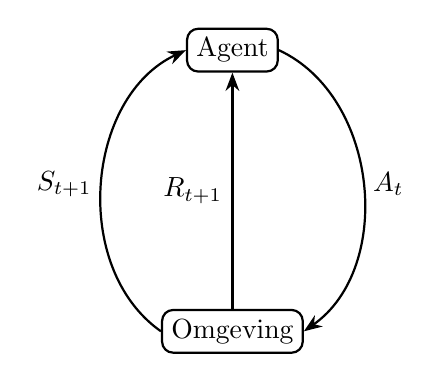
\begin{tikzpicture}[auto, thick, node distance=2cm,>=Stealth]
        \node[draw, rectangle, rounded corners] (agent) {Agent};
        \node[draw, rectangle, rounded corners, below=of agent, yshift=-1cm] (environment) {Omgeving};

        % Action arrow with adjusted bend
        \draw[->] (agent.east) to[bend left=60] node[midway, right] {$A_t$} (environment.east);

        % State arrow with adjusted text position
        \draw[->] (environment.north) to node[midway, left] {$R_{t+1}$} (agent.south);

        % Reward arrow with adjusted text position
        \draw[->] (environment.west) to[bend left=60] node[midway, left] {$S_{t+1}$} (agent.west);
    \end{tikzpicture}
    \caption{Reinforcement learning interactiemodel tussen agent en omgeving via acties, toestanden en beloningen.}
    \label{fig:rl_model}
\end{figure}
\subsection{Markov Decision Process (MDP)}

MDP werkt onder de Markov-aanname, wat betekent dat de volgende toestand en
beloning alleen afhangen van het huidige toestand-actiepaar en niet van enige
eerdere geschiedenis. Deze eigenschap vereenvoudigt het besluitvormingsmodel
door zich alleen te concentreren op de huidige situatie.

Voorbeeld van een MDP:
\begin{itemize}
    \item \textbf{Snake}: De toekomstige toestand (positie van de slang en voedsel) is volledig bepaald door de huidige toestand (huidige positie en locatie van het voedsel) en de actie (richting van beweging) zonder afhankelijk te zijn van de geschiedenis van eerdere bewegingen.
\end{itemize}

Voorbeeld van geen MDP:
\begin{itemize}
    \item \textbf{Poker}: De beslissingen in poker zijn afhankelijk van niet alleen de huidige hand, maar ook van de geschiedenis van inzetten en het gedrag van andere spelers in vorige rondes.
\end{itemize}

In een MDP gaat een agent verder in tijdstappen \(t = 0, 1, 2, \ldots, T\) waar
de horizon \(T\) zowel eindig als oneindig kan zijn.

\section{Onderzoeksplan en -overzicht}

\subsection{Taakverdeling en Planning}
De taken zullen als volgt worden verdeeld:
\begin{enumerate}
    \item \textbf{Theoretisch kader opstellen}: Inlezen en samenvatten van de beschikbare literatuur over RL-algoritmes en hun toepassing in games.
    \item \textbf{Selectie van spellen en algoritmes}: Identificatie en selectie van spellen (\textit{Snake}, \textit{Mario Super Bros}, autoracen) en RL-algoritmes (met nadruk op DQL).
    \item \textbf{Experimenten uitvoeren}: Toepassing van de geselecteerde RL-algoritmes op de gekozen spellen en het verzamelen van prestatiegegevens.
    \item \textbf{Data-analyse}: Analyseren van de prestaties van de RL-algoritmes in relatie tot de spelkenmerken.
    \item \textbf{Conclusies trekken en verslag schrijven}: Samenstellen van het eindrapport waarin de resultaten en conclusies worden gepresenteerd.
\end{enumerate}

\subsection{Planning}
T = Gechatte tijd pp \\ \small

\begin{tabular}{|>{\raggedright}m{6cm}|>{\raggedright}m{2.3cm}|>{\raggedright}m{1.4cm}|>{\raggedright}m{2.3cm}|>{\raggedright\arraybackslash}m{2cm}|}
    \hline
    \textbf{Taak}                     & \textbf{Persoon} & \textbf{T(uur)} & \textbf{Startdatum} & \textbf{Deadline} \\ \hline
    Taakverdeling \& planning         & Alle             & 3               & 30/08/2024          & 04/09/2024        \\
    PWS voorstel maken                & Matthijs         & 3               & 04/09/2024          & 06/09/2024        \\
    PWS voorstel inleveren            & 1p               & nvt             & 06/09/2024          & 06/09/2024        \\
    Inlezen in onderwerp              & Alle             & 10              & 06/09/2024          & 20/09/2024        \\
    Theoretisch kader opstellen       & Matthijs         & 20              & 20/09/2024          & 04/10/2024        \\
    Deelvraag 1 beantwoorden          & 1p               & 10              & 20/09/2024          & 04/10/2024        \\
    Deelvraag 2 beantwoorden          & 1p               & 10              & 20/09/2024          & 04/10/2024        \\
    Deelvraag 3 beantwoorden          & 1p               & 15              & 04/10/2024          & 18/10/2024        \\
    Experiment 1 uitvoeren            & Matthijs         & 20              & 04/10/2024          & 18/10/2024        \\
    Resultaten Experiment 1 verwerken & 1p               & 5               & 18/10/2024          & 25/10/2024        \\
    Experiment 2 uitvoeren            & Matthijs         & 10              & 18/10/2024          & 25/10/2024        \\
    Herfstvakantie en Toetsweek 1     & Alle             & nvt             & 25/10/2024          & 19/11/2024        \\
    Eerste versie PWS maken           & 1p, Matthijs     & 8               & 20/11/2024          & 29/11/2024        \\
    Eerste versie inleveren           & 1p               & nvt             & 29/11/2024          & 29/11/2024        \\
    Resultaten Experiment 2 verwerken & 1p               & 5               & 20/11/2024          & 29/11/2024        \\
    Experiment 3 uitvoeren            & Matthijs         & 10              & 29/11/2024          & 13/12/2024        \\
    Resultaten Experiment 3 verwerken & 1p               & 5               & 13/12/2024          & 20/12/2024        \\
    Kerstvakantie                     & Alle             & nvt             & 21/12/2024          & 05/01/2025        \\
    Resultaten                        & 1p               & 3               & 05/01/2024          & 13/01/2025        \\
    Toetsweek 2                       & Alle             & nvt             & 13/01/2024          & 31/01/2025        \\
    Conclusie                         & 1p               & 10              & 31/01/2024          & 16/02/2025        \\
    Onderzoeksmethode                 & Matthijs         & 3               & 31/01/2024          & 16/02/2025        \\
    Discussie                         & 1p               & 3               & 31/01/2024          & 16/02/2025        \\
    Voorwoord                         & 1p               & 3               & 31/01/2024          & 16/02/2025        \\
    Referentielijst                   & 1p               & 3               & 31/01/2024          & 16/02/2025        \\
    Nakijken van alle hoofdstukken    & Alle             & 3               & 16/02/2024          & 19/02/2025        \\
    Eindversie maken                  & Matthijs         & 2               & 19/02/2024          & 21/02/2025        \\
    Eindversie inleveren              & 1p               & nvt             & 21/02/2024          & 21/02/2025        \\
    \hline

\end{tabular}
\section{Bronvermelding}
Voor de theoretische onderbouwing en achtergrondinformatie zullen de volgende
bronnen worden gebruikt:
\begin{itemize}
    \item \textit{Reinforcement Learning: An Introduction} door Andrew Barto en Richard S. Sutton.
          \begin{itemize}
              \item \url{https://web.stanford.edu/class/psych209/Readings/SuttonBartoIPRLBook2ndEd.pdf}
              \item \url{http://incompleteideas.net/book/RLbook2020.pdf}
          \end{itemize}
    \item Stanford CS234 Winter 2019: \textit{Reinforcement Learning} (15 colleges).
          \begin{itemize}
              \item \url{https://www.youtube.com/playlist?list=PLoROMvodv4rOSOPzutgyCTapiGlY2Nd8u}
          \end{itemize}
    \item \textit{Spinning Up in Deep RL} door OpenAI.
          \begin{itemize}
              \item \url{https://spinningup.openai.com/en/latest/index.html}
          \end{itemize}

    \item Yunhao Tang 2021: \textit{Deep Reinforcement Learning}.
          \begin{itemize}
              \item \url{https://academiccommons.columbia.edu/doi/10.7916/d8-7b4y-dk07}
              \item \url{https://web.archive.org/web/20240429102051/https://academiccommons.columbia.edu/doi/10.7916/d8-y0tc-h725/download}
          \end{itemize}
\end{itemize}
Daarnaast zullen eerdere PWS-projecten worden geraadpleegd, zoals:
\begin{itemize}
    \item \textit{Een kunstmatige opsporing van longkanker} (2023) - KNAW. \\
          \url{https://storage.knaw.nl/2023-06/profielwerkstuk-2023-een-kunstmatige-opsporing-van-longkanker.pdf}
    \item \textit{File en nog eens file} (2023) - KNAW. \\
          \url{https://storage.knaw.nl/2023-06/pws-file-file-en-nog-eens-file.pdf}
\end{itemize}

\end{document}
